
% Default to the notebook output style

    


% Inherit from the specified cell style.




    
\documentclass[11pt]{ctexart}

    
    
    \usepackage[T1]{fontenc}
    % Nicer default font (+ math font) than Computer Modern for most use cases
    \usepackage{mathpazo}

    % Basic figure setup, for now with no caption control since it's done
    % automatically by Pandoc (which extracts ![](path) syntax from Markdown).
    \usepackage{graphicx}
    % We will generate all images so they have a width \maxwidth. This means
    % that they will get their normal width if they fit onto the page, but
    % are scaled down if they would overflow the margins.
    \makeatletter
    \def\maxwidth{\ifdim\Gin@nat@width>\linewidth\linewidth
    \else\Gin@nat@width\fi}
    \makeatother
    \let\Oldincludegraphics\includegraphics
    % Set max figure width to be 80% of text width, for now hardcoded.
    \renewcommand{\includegraphics}[1]{\Oldincludegraphics[width=.8\maxwidth]{#1}}
    % Ensure that by default, figures have no caption (until we provide a
    % proper Figure object with a Caption API and a way to capture that
    % in the conversion process - todo).
    \usepackage{caption}
    \DeclareCaptionLabelFormat{nolabel}{}
    \captionsetup{labelformat=nolabel}

    \usepackage{adjustbox} % Used to constrain images to a maximum size 
    \usepackage{xcolor} % Allow colors to be defined
    \usepackage{enumerate} % Needed for markdown enumerations to work
    \usepackage{geometry} % Used to adjust the document margins
    \usepackage{amsmath} % Equations
    \usepackage{amssymb} % Equations
    \usepackage{textcomp} % defines textquotesingle
    % Hack from http://tex.stackexchange.com/a/47451/13684:
    \AtBeginDocument{%
        \def\PYZsq{\textquotesingle}% Upright quotes in Pygmentized code
    }
    \usepackage{upquote} % Upright quotes for verbatim code
    \usepackage{eurosym} % defines \euro
    \usepackage[mathletters]{ucs} % Extended unicode (utf-8) support
    \usepackage[utf8x]{inputenc} % Allow utf-8 characters in the tex document
    \usepackage{fancyvrb} % verbatim replacement that allows latex
    \usepackage{grffile} % extends the file name processing of package graphics 
                         % to support a larger range 
    % The hyperref package gives us a pdf with properly built
    % internal navigation ('pdf bookmarks' for the table of contents,
    % internal cross-reference links, web links for URLs, etc.)
    \usepackage{hyperref}
    \usepackage{longtable} % longtable support required by pandoc >1.10
    \usepackage{booktabs}  % table support for pandoc > 1.12.2
    \usepackage[inline]{enumitem} % IRkernel/repr support (it uses the enumerate* environment)
    \usepackage[normalem]{ulem} % ulem is needed to support strikethroughs (\sout)
                                % normalem makes italics be italics, not underlines
    

    
    
    % Colors for the hyperref package
    \definecolor{urlcolor}{rgb}{0,.145,.698}
    \definecolor{linkcolor}{rgb}{.71,0.21,0.01}
    \definecolor{citecolor}{rgb}{.12,.54,.11}

    % ANSI colors
    \definecolor{ansi-black}{HTML}{3E424D}
    \definecolor{ansi-black-intense}{HTML}{282C36}
    \definecolor{ansi-red}{HTML}{E75C58}
    \definecolor{ansi-red-intense}{HTML}{B22B31}
    \definecolor{ansi-green}{HTML}{00A250}
    \definecolor{ansi-green-intense}{HTML}{007427}
    \definecolor{ansi-yellow}{HTML}{DDB62B}
    \definecolor{ansi-yellow-intense}{HTML}{B27D12}
    \definecolor{ansi-blue}{HTML}{208FFB}
    \definecolor{ansi-blue-intense}{HTML}{0065CA}
    \definecolor{ansi-magenta}{HTML}{D160C4}
    \definecolor{ansi-magenta-intense}{HTML}{A03196}
    \definecolor{ansi-cyan}{HTML}{60C6C8}
    \definecolor{ansi-cyan-intense}{HTML}{258F8F}
    \definecolor{ansi-white}{HTML}{C5C1B4}
    \definecolor{ansi-white-intense}{HTML}{A1A6B2}

    % commands and environments needed by pandoc snippets
    % extracted from the output of `pandoc -s`
    \providecommand{\tightlist}{%
      \setlength{\itemsep}{0pt}\setlength{\parskip}{0pt}}
    \DefineVerbatimEnvironment{Highlighting}{Verbatim}{commandchars=\\\{\}}
    % Add ',fontsize=\small' for more characters per line
    \newenvironment{Shaded}{}{}
    \newcommand{\KeywordTok}[1]{\textcolor[rgb]{0.00,0.44,0.13}{\textbf{{#1}}}}
    \newcommand{\DataTypeTok}[1]{\textcolor[rgb]{0.56,0.13,0.00}{{#1}}}
    \newcommand{\DecValTok}[1]{\textcolor[rgb]{0.25,0.63,0.44}{{#1}}}
    \newcommand{\BaseNTok}[1]{\textcolor[rgb]{0.25,0.63,0.44}{{#1}}}
    \newcommand{\FloatTok}[1]{\textcolor[rgb]{0.25,0.63,0.44}{{#1}}}
    \newcommand{\CharTok}[1]{\textcolor[rgb]{0.25,0.44,0.63}{{#1}}}
    \newcommand{\StringTok}[1]{\textcolor[rgb]{0.25,0.44,0.63}{{#1}}}
    \newcommand{\CommentTok}[1]{\textcolor[rgb]{0.38,0.63,0.69}{\textit{{#1}}}}
    \newcommand{\OtherTok}[1]{\textcolor[rgb]{0.00,0.44,0.13}{{#1}}}
    \newcommand{\AlertTok}[1]{\textcolor[rgb]{1.00,0.00,0.00}{\textbf{{#1}}}}
    \newcommand{\FunctionTok}[1]{\textcolor[rgb]{0.02,0.16,0.49}{{#1}}}
    \newcommand{\RegionMarkerTok}[1]{{#1}}
    \newcommand{\ErrorTok}[1]{\textcolor[rgb]{1.00,0.00,0.00}{\textbf{{#1}}}}
    \newcommand{\NormalTok}[1]{{#1}}
    
    % Additional commands for more recent versions of Pandoc
    \newcommand{\ConstantTok}[1]{\textcolor[rgb]{0.53,0.00,0.00}{{#1}}}
    \newcommand{\SpecialCharTok}[1]{\textcolor[rgb]{0.25,0.44,0.63}{{#1}}}
    \newcommand{\VerbatimStringTok}[1]{\textcolor[rgb]{0.25,0.44,0.63}{{#1}}}
    \newcommand{\SpecialStringTok}[1]{\textcolor[rgb]{0.73,0.40,0.53}{{#1}}}
    \newcommand{\ImportTok}[1]{{#1}}
    \newcommand{\DocumentationTok}[1]{\textcolor[rgb]{0.73,0.13,0.13}{\textit{{#1}}}}
    \newcommand{\AnnotationTok}[1]{\textcolor[rgb]{0.38,0.63,0.69}{\textbf{\textit{{#1}}}}}
    \newcommand{\CommentVarTok}[1]{\textcolor[rgb]{0.38,0.63,0.69}{\textbf{\textit{{#1}}}}}
    \newcommand{\VariableTok}[1]{\textcolor[rgb]{0.10,0.09,0.49}{{#1}}}
    \newcommand{\ControlFlowTok}[1]{\textcolor[rgb]{0.00,0.44,0.13}{\textbf{{#1}}}}
    \newcommand{\OperatorTok}[1]{\textcolor[rgb]{0.40,0.40,0.40}{{#1}}}
    \newcommand{\BuiltInTok}[1]{{#1}}
    \newcommand{\ExtensionTok}[1]{{#1}}
    \newcommand{\PreprocessorTok}[1]{\textcolor[rgb]{0.74,0.48,0.00}{{#1}}}
    \newcommand{\AttributeTok}[1]{\textcolor[rgb]{0.49,0.56,0.16}{{#1}}}
    \newcommand{\InformationTok}[1]{\textcolor[rgb]{0.38,0.63,0.69}{\textbf{\textit{{#1}}}}}
    \newcommand{\WarningTok}[1]{\textcolor[rgb]{0.38,0.63,0.69}{\textbf{\textit{{#1}}}}}
    
    
    % Define a nice break command that doesn't care if a line doesn't already
    % exist.
    \def\br{\hspace*{\fill} \\* }
    % Math Jax compatability definitions
    \def\gt{>}
    \def\lt{<}
    % Document parameters
    \title{PandasBasic}
    
    
    

    % Pygments definitions
    
\makeatletter
\def\PY@reset{\let\PY@it=\relax \let\PY@bf=\relax%
    \let\PY@ul=\relax \let\PY@tc=\relax%
    \let\PY@bc=\relax \let\PY@ff=\relax}
\def\PY@tok#1{\csname PY@tok@#1\endcsname}
\def\PY@toks#1+{\ifx\relax#1\empty\else%
    \PY@tok{#1}\expandafter\PY@toks\fi}
\def\PY@do#1{\PY@bc{\PY@tc{\PY@ul{%
    \PY@it{\PY@bf{\PY@ff{#1}}}}}}}
\def\PY#1#2{\PY@reset\PY@toks#1+\relax+\PY@do{#2}}

\expandafter\def\csname PY@tok@gr\endcsname{\def\PY@tc##1{\textcolor[rgb]{1.00,0.00,0.00}{##1}}}
\expandafter\def\csname PY@tok@mh\endcsname{\def\PY@tc##1{\textcolor[rgb]{0.40,0.40,0.40}{##1}}}
\expandafter\def\csname PY@tok@sr\endcsname{\def\PY@tc##1{\textcolor[rgb]{0.73,0.40,0.53}{##1}}}
\expandafter\def\csname PY@tok@sa\endcsname{\def\PY@tc##1{\textcolor[rgb]{0.73,0.13,0.13}{##1}}}
\expandafter\def\csname PY@tok@gt\endcsname{\def\PY@tc##1{\textcolor[rgb]{0.00,0.27,0.87}{##1}}}
\expandafter\def\csname PY@tok@nn\endcsname{\let\PY@bf=\textbf\def\PY@tc##1{\textcolor[rgb]{0.00,0.00,1.00}{##1}}}
\expandafter\def\csname PY@tok@kp\endcsname{\def\PY@tc##1{\textcolor[rgb]{0.00,0.50,0.00}{##1}}}
\expandafter\def\csname PY@tok@nb\endcsname{\def\PY@tc##1{\textcolor[rgb]{0.00,0.50,0.00}{##1}}}
\expandafter\def\csname PY@tok@s1\endcsname{\def\PY@tc##1{\textcolor[rgb]{0.73,0.13,0.13}{##1}}}
\expandafter\def\csname PY@tok@gs\endcsname{\let\PY@bf=\textbf}
\expandafter\def\csname PY@tok@kt\endcsname{\def\PY@tc##1{\textcolor[rgb]{0.69,0.00,0.25}{##1}}}
\expandafter\def\csname PY@tok@kc\endcsname{\let\PY@bf=\textbf\def\PY@tc##1{\textcolor[rgb]{0.00,0.50,0.00}{##1}}}
\expandafter\def\csname PY@tok@cp\endcsname{\def\PY@tc##1{\textcolor[rgb]{0.74,0.48,0.00}{##1}}}
\expandafter\def\csname PY@tok@gi\endcsname{\def\PY@tc##1{\textcolor[rgb]{0.00,0.63,0.00}{##1}}}
\expandafter\def\csname PY@tok@bp\endcsname{\def\PY@tc##1{\textcolor[rgb]{0.00,0.50,0.00}{##1}}}
\expandafter\def\csname PY@tok@mi\endcsname{\def\PY@tc##1{\textcolor[rgb]{0.40,0.40,0.40}{##1}}}
\expandafter\def\csname PY@tok@ss\endcsname{\def\PY@tc##1{\textcolor[rgb]{0.10,0.09,0.49}{##1}}}
\expandafter\def\csname PY@tok@s\endcsname{\def\PY@tc##1{\textcolor[rgb]{0.73,0.13,0.13}{##1}}}
\expandafter\def\csname PY@tok@sd\endcsname{\let\PY@it=\textit\def\PY@tc##1{\textcolor[rgb]{0.73,0.13,0.13}{##1}}}
\expandafter\def\csname PY@tok@c\endcsname{\let\PY@it=\textit\def\PY@tc##1{\textcolor[rgb]{0.25,0.50,0.50}{##1}}}
\expandafter\def\csname PY@tok@nf\endcsname{\def\PY@tc##1{\textcolor[rgb]{0.00,0.00,1.00}{##1}}}
\expandafter\def\csname PY@tok@vm\endcsname{\def\PY@tc##1{\textcolor[rgb]{0.10,0.09,0.49}{##1}}}
\expandafter\def\csname PY@tok@mo\endcsname{\def\PY@tc##1{\textcolor[rgb]{0.40,0.40,0.40}{##1}}}
\expandafter\def\csname PY@tok@ow\endcsname{\let\PY@bf=\textbf\def\PY@tc##1{\textcolor[rgb]{0.67,0.13,1.00}{##1}}}
\expandafter\def\csname PY@tok@no\endcsname{\def\PY@tc##1{\textcolor[rgb]{0.53,0.00,0.00}{##1}}}
\expandafter\def\csname PY@tok@gd\endcsname{\def\PY@tc##1{\textcolor[rgb]{0.63,0.00,0.00}{##1}}}
\expandafter\def\csname PY@tok@gp\endcsname{\let\PY@bf=\textbf\def\PY@tc##1{\textcolor[rgb]{0.00,0.00,0.50}{##1}}}
\expandafter\def\csname PY@tok@sb\endcsname{\def\PY@tc##1{\textcolor[rgb]{0.73,0.13,0.13}{##1}}}
\expandafter\def\csname PY@tok@gh\endcsname{\let\PY@bf=\textbf\def\PY@tc##1{\textcolor[rgb]{0.00,0.00,0.50}{##1}}}
\expandafter\def\csname PY@tok@o\endcsname{\def\PY@tc##1{\textcolor[rgb]{0.40,0.40,0.40}{##1}}}
\expandafter\def\csname PY@tok@sc\endcsname{\def\PY@tc##1{\textcolor[rgb]{0.73,0.13,0.13}{##1}}}
\expandafter\def\csname PY@tok@nv\endcsname{\def\PY@tc##1{\textcolor[rgb]{0.10,0.09,0.49}{##1}}}
\expandafter\def\csname PY@tok@kd\endcsname{\let\PY@bf=\textbf\def\PY@tc##1{\textcolor[rgb]{0.00,0.50,0.00}{##1}}}
\expandafter\def\csname PY@tok@si\endcsname{\let\PY@bf=\textbf\def\PY@tc##1{\textcolor[rgb]{0.73,0.40,0.53}{##1}}}
\expandafter\def\csname PY@tok@il\endcsname{\def\PY@tc##1{\textcolor[rgb]{0.40,0.40,0.40}{##1}}}
\expandafter\def\csname PY@tok@m\endcsname{\def\PY@tc##1{\textcolor[rgb]{0.40,0.40,0.40}{##1}}}
\expandafter\def\csname PY@tok@k\endcsname{\let\PY@bf=\textbf\def\PY@tc##1{\textcolor[rgb]{0.00,0.50,0.00}{##1}}}
\expandafter\def\csname PY@tok@kn\endcsname{\let\PY@bf=\textbf\def\PY@tc##1{\textcolor[rgb]{0.00,0.50,0.00}{##1}}}
\expandafter\def\csname PY@tok@ne\endcsname{\let\PY@bf=\textbf\def\PY@tc##1{\textcolor[rgb]{0.82,0.25,0.23}{##1}}}
\expandafter\def\csname PY@tok@c1\endcsname{\let\PY@it=\textit\def\PY@tc##1{\textcolor[rgb]{0.25,0.50,0.50}{##1}}}
\expandafter\def\csname PY@tok@s2\endcsname{\def\PY@tc##1{\textcolor[rgb]{0.73,0.13,0.13}{##1}}}
\expandafter\def\csname PY@tok@nl\endcsname{\def\PY@tc##1{\textcolor[rgb]{0.63,0.63,0.00}{##1}}}
\expandafter\def\csname PY@tok@sh\endcsname{\def\PY@tc##1{\textcolor[rgb]{0.73,0.13,0.13}{##1}}}
\expandafter\def\csname PY@tok@vg\endcsname{\def\PY@tc##1{\textcolor[rgb]{0.10,0.09,0.49}{##1}}}
\expandafter\def\csname PY@tok@kr\endcsname{\let\PY@bf=\textbf\def\PY@tc##1{\textcolor[rgb]{0.00,0.50,0.00}{##1}}}
\expandafter\def\csname PY@tok@fm\endcsname{\def\PY@tc##1{\textcolor[rgb]{0.00,0.00,1.00}{##1}}}
\expandafter\def\csname PY@tok@gu\endcsname{\let\PY@bf=\textbf\def\PY@tc##1{\textcolor[rgb]{0.50,0.00,0.50}{##1}}}
\expandafter\def\csname PY@tok@se\endcsname{\let\PY@bf=\textbf\def\PY@tc##1{\textcolor[rgb]{0.73,0.40,0.13}{##1}}}
\expandafter\def\csname PY@tok@nd\endcsname{\def\PY@tc##1{\textcolor[rgb]{0.67,0.13,1.00}{##1}}}
\expandafter\def\csname PY@tok@ge\endcsname{\let\PY@it=\textit}
\expandafter\def\csname PY@tok@sx\endcsname{\def\PY@tc##1{\textcolor[rgb]{0.00,0.50,0.00}{##1}}}
\expandafter\def\csname PY@tok@cm\endcsname{\let\PY@it=\textit\def\PY@tc##1{\textcolor[rgb]{0.25,0.50,0.50}{##1}}}
\expandafter\def\csname PY@tok@w\endcsname{\def\PY@tc##1{\textcolor[rgb]{0.73,0.73,0.73}{##1}}}
\expandafter\def\csname PY@tok@vc\endcsname{\def\PY@tc##1{\textcolor[rgb]{0.10,0.09,0.49}{##1}}}
\expandafter\def\csname PY@tok@ni\endcsname{\let\PY@bf=\textbf\def\PY@tc##1{\textcolor[rgb]{0.60,0.60,0.60}{##1}}}
\expandafter\def\csname PY@tok@err\endcsname{\def\PY@bc##1{\setlength{\fboxsep}{0pt}\fcolorbox[rgb]{1.00,0.00,0.00}{1,1,1}{\strut ##1}}}
\expandafter\def\csname PY@tok@nt\endcsname{\let\PY@bf=\textbf\def\PY@tc##1{\textcolor[rgb]{0.00,0.50,0.00}{##1}}}
\expandafter\def\csname PY@tok@nc\endcsname{\let\PY@bf=\textbf\def\PY@tc##1{\textcolor[rgb]{0.00,0.00,1.00}{##1}}}
\expandafter\def\csname PY@tok@mb\endcsname{\def\PY@tc##1{\textcolor[rgb]{0.40,0.40,0.40}{##1}}}
\expandafter\def\csname PY@tok@ch\endcsname{\let\PY@it=\textit\def\PY@tc##1{\textcolor[rgb]{0.25,0.50,0.50}{##1}}}
\expandafter\def\csname PY@tok@cs\endcsname{\let\PY@it=\textit\def\PY@tc##1{\textcolor[rgb]{0.25,0.50,0.50}{##1}}}
\expandafter\def\csname PY@tok@dl\endcsname{\def\PY@tc##1{\textcolor[rgb]{0.73,0.13,0.13}{##1}}}
\expandafter\def\csname PY@tok@go\endcsname{\def\PY@tc##1{\textcolor[rgb]{0.53,0.53,0.53}{##1}}}
\expandafter\def\csname PY@tok@vi\endcsname{\def\PY@tc##1{\textcolor[rgb]{0.10,0.09,0.49}{##1}}}
\expandafter\def\csname PY@tok@cpf\endcsname{\let\PY@it=\textit\def\PY@tc##1{\textcolor[rgb]{0.25,0.50,0.50}{##1}}}
\expandafter\def\csname PY@tok@na\endcsname{\def\PY@tc##1{\textcolor[rgb]{0.49,0.56,0.16}{##1}}}
\expandafter\def\csname PY@tok@mf\endcsname{\def\PY@tc##1{\textcolor[rgb]{0.40,0.40,0.40}{##1}}}

\def\PYZbs{\char`\\}
\def\PYZus{\char`\_}
\def\PYZob{\char`\{}
\def\PYZcb{\char`\}}
\def\PYZca{\char`\^}
\def\PYZam{\char`\&}
\def\PYZlt{\char`\<}
\def\PYZgt{\char`\>}
\def\PYZsh{\char`\#}
\def\PYZpc{\char`\%}
\def\PYZdl{\char`\$}
\def\PYZhy{\char`\-}
\def\PYZsq{\char`\'}
\def\PYZdq{\char`\"}
\def\PYZti{\char`\~}
% for compatibility with earlier versions
\def\PYZat{@}
\def\PYZlb{[}
\def\PYZrb{]}
\makeatother


    % Exact colors from NB
    \definecolor{incolor}{rgb}{0.0, 0.0, 0.5}
    \definecolor{outcolor}{rgb}{0.545, 0.0, 0.0}



    
    % Prevent overflowing lines due to hard-to-break entities
    \sloppy 
    % Setup hyperref package
    \hypersetup{
      breaklinks=true,  % so long urls are correctly broken across lines
      colorlinks=true,
      urlcolor=urlcolor,
      linkcolor=linkcolor,
      citecolor=citecolor,
      }
    % Slightly bigger margins than the latex defaults
    
    \geometry{verbose,tmargin=1in,bmargin=1in,lmargin=1in,rmargin=1in}
    
    

    \begin{document}
    
    
    \maketitle
    
    

    
    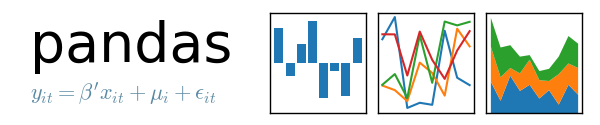
\includegraphics{pandas_logo.png}

\hypertarget{pandasux57faux672cux4f7fux7528}{%
\section{Pandas基本使用}\label{pandasux57faux672cux4f7fux7528}}

\hypertarget{ux4ecbux7d39}{%
\subsection{介紹}\label{ux4ecbux7d39}}

專門拿來處理表格的函式庫,一生懸命只為了處理表格而生

\hypertarget{ux7528ux9014}{%
\subsection{用途}\label{ux7528ux9014}}

\begin{enumerate}
\def\labelenumi{\arabic{enumi}.}
\tightlist
\item
  處理各種表格(csv, excel\ldots{}等等)
\item
  拿來表示機器學習的資料集(每個列就是一個物品,每個行代表物品的每個特徵
\item
  可以快速結合常用的繪圖函式庫,直接畫出漂亮的圖形
\end{enumerate}

\hypertarget{ux5b89ux88ddux65b9ux6cd5}{%
\subsection{安裝方法}\label{ux5b89ux88ddux65b9ux6cd5}}

\begin{enumerate}
\def\labelenumi{\arabic{enumi}.}
\tightlist
\item
  使用PyCharm: PyCharm -\textgreater{} Settings -\textgreater{} Project
  -\textgreater{} Project Interpreter -\textgreater{} + -\textgreater{}
  (搜索)pandas -\textgreater{} Install Packages
\item
  使用命令列: cd到你安裝Python的資料夾 -\textgreater{} 輸入 python -m
  pip install pandas
\end{enumerate}

\hypertarget{ux5b98ux65b9ux6587ux4ef6}{%
\subsection{官方文件}\label{ux5b98ux65b9ux6587ux4ef6}}

http://pandas.pydata.org/pandas-docs/stable/

\hypertarget{ux53efux4ee5ux8655ux7406ux7684ux8868ux683cux5f62ux5f0f}{%
\subsection{可以處理的表格形式}\label{ux53efux4ee5ux8655ux7406ux7684ux8868ux683cux5f62ux5f0f}}

http://pandas.pydata.org/pandas-docs/stable/io.html

\hypertarget{ux76eeux6a19}{%
\subsection{目標}\label{ux76eeux6a19}}

我們使用Kaggle的TED資料集來教你Pandas的基本操作

\hypertarget{ux8cc7ux6599ux96c6ux4f4dux7f6e}{%
\subsection{資料集位置}\label{ux8cc7ux6599ux96c6ux4f4dux7f6e}}

https://www.kaggle.com/rounakbanik/ted-talks

\begin{enumerate}
\def\labelenumi{\arabic{enumi}.}
\tightlist
\item
  需要登入才能下載
\item
  只取裡面的ted\_main.csv來做分析
\end{enumerate}

\hypertarget{pandasux57faux672cux8cc7ux6599}{%
\subsection{✔ Pandas基本資料}\label{pandasux57faux672cux8cc7ux6599}}

\begin{enumerate}
\def\labelenumi{\arabic{enumi}.}
\tightlist
\item
  多個行 * 多個列 -\textgreater{} DataFrame
\item
  一個行 * 多個列 或者 一個列 * 多個行 -\textgreater{} Series
\end{enumerate}

    \begin{Verbatim}[commandchars=\\\{\}]
{\color{incolor}In [{\color{incolor}1}]:} \PY{k+kn}{import} \PY{n+nn}{pandas} \PY{k}{as} \PY{n+nn}{pd}
        \PY{c+c1}{\PYZsh{} 為了顯示的漂亮, 我刻意的把印出來的row和column只顯示六個, 大家練習的時候可以去掉下面兩行}
        \PY{n}{pd}\PY{o}{.}\PY{n}{set\PYZus{}option}\PY{p}{(}\PY{l+s+s1}{\PYZsq{}}\PY{l+s+s1}{display.max\PYZus{}rows}\PY{l+s+s1}{\PYZsq{}}\PY{p}{,} \PY{l+m+mi}{6}\PY{p}{)}
        \PY{n}{pd}\PY{o}{.}\PY{n}{set\PYZus{}option}\PY{p}{(}\PY{l+s+s1}{\PYZsq{}}\PY{l+s+s1}{display.max\PYZus{}columns}\PY{l+s+s1}{\PYZsq{}}\PY{p}{,} \PY{l+m+mi}{6}\PY{p}{)}
\end{Verbatim}


    \hypertarget{ux8b80ux53d6ux8868ux683cux64cdux4f5c}{%
\subsection{✔ 讀取表格操作}\label{ux8b80ux53d6ux8868ux683cux64cdux4f5c}}

使用read\_表格形式來讀取,
記得最好明確表示用utf-8來讀取網站檔案(網路上的檔案通常使用utf-8來儲存)

\textbf{注意:}
如果是windows的一些檔案,內建的儲存編碼是ANSI,用utf-8會失效,我們留待編碼篇好好說

\hypertarget{read_csvux91cdux8981ux53c3ux6578}{%
\subsubsection{read\_csv重要參數:}\label{read_csvux91cdux8981ux53c3ux6578}}

\begin{enumerate}
\def\labelenumi{\arabic{enumi}.}
\tightlist
\item
  必要參數: 檔案位置
\item
  選用參數(有預設值): 讀取使用編碼
\end{enumerate}

\hypertarget{read_csvux56deux50b3ux503c}{%
\subsubsection{read\_csv回傳值:}\label{read_csvux56deux50b3ux503c}}

DataFrame

    \begin{Verbatim}[commandchars=\\\{\}]
{\color{incolor}In [{\color{incolor}2}]:} \PY{n}{df} \PY{o}{=} \PY{n}{pd}\PY{o}{.}\PY{n}{read\PYZus{}csv}\PY{p}{(}\PY{l+s+s2}{\PYZdq{}}\PY{l+s+s2}{ted\PYZus{}main.csv}\PY{l+s+s2}{\PYZdq{}}\PY{p}{,} \PY{n}{encoding} \PY{o}{=} \PY{l+s+s2}{\PYZdq{}}\PY{l+s+s2}{utf\PYZhy{}8}\PY{l+s+s2}{\PYZdq{}}\PY{p}{)}
        \PY{n}{df}
\end{Verbatim}


\begin{Verbatim}[commandchars=\\\{\}]
{\color{outcolor}Out[{\color{outcolor}2}]:}       comments                                        description  duration  \textbackslash{}
        0         4553  Sir Ken Robinson makes an entertaining and pro{\ldots}      1164   
        1          265  With the same humor and humanity he exuded in {\ldots}       977   
        2          124  New York Times columnist David Pogue takes aim{\ldots}      1286   
        {\ldots}        {\ldots}                                                {\ldots}       {\ldots}   
        2547        10  Science fiction visions of the future show us {\ldots}       651   
        2548        32  In an unmissable talk about race and politics {\ldots}      1100   
        2549         8  With more than half of the world population li{\ldots}       519   
        
                {\ldots}                                                 title  \textbackslash{}
        0       {\ldots}                           Do schools kill creativity?   
        1       {\ldots}                           Averting the climate crisis   
        2       {\ldots}                                      Simplicity sells   
        {\ldots}     {\ldots}                                                   {\ldots}   
        2547    {\ldots}     What intelligent machines can learn from a sch{\ldots}   
        2548    {\ldots}          A black man goes undercover in the alt-right   
        2549    {\ldots}     How a video game might help us build better ci{\ldots}   
        
                                                            url     views  
        0     https://www.ted.com/talks/ken\_robinson\_says\_sc{\ldots}  47227110  
        1     https://www.ted.com/talks/al\_gore\_on\_averting\_{\ldots}   3200520  
        2     https://www.ted.com/talks/david\_pogue\_says\_sim{\ldots}   1636292  
        {\ldots}                                                 {\ldots}       {\ldots}  
        2547  https://www.ted.com/talks/radhika\_nagpal\_what\_{\ldots}    375647  
        2548  https://www.ted.com/talks/theo\_e\_j\_wilson\_a\_bl{\ldots}    419309  
        2549  https://www.ted.com/talks/karoliina\_korppoo\_ho{\ldots}    391721  
        
        [2550 rows x 17 columns]
\end{Verbatim}
            
    \hypertarget{dataframeux5927ux5c0f}{%
\subsection{✔ DataFrame大小}\label{dataframeux5927ux5c0f}}

\begin{enumerate}
\def\labelenumi{\arabic{enumi}.}
\tightlist
\item
  由於我們有兩個維度,所以以前習慣的len不能使用了,我們要使用.shape來取得兩個維度
\item
  .shape是一個tuple,所以第一個元素{[}0{]}就是你的列數,第二個元素{[}1{]}就是你的行數
\end{enumerate}

    \begin{Verbatim}[commandchars=\\\{\}]
{\color{incolor}In [{\color{incolor}3}]:} \PY{n}{df}\PY{o}{.}\PY{n}{shape}
\end{Verbatim}


\begin{Verbatim}[commandchars=\\\{\}]
{\color{outcolor}Out[{\color{outcolor}3}]:} (2550, 17)
\end{Verbatim}
            
    \hypertarget{ux8868ux683cux884cux7be9ux9078}{%
\subsection{✔ 表格行篩選}\label{ux8868ux683cux884cux7be9ux9078}}

篩選行的時候,我們就像在操作字典一樣,對你的DataFrame加上 {[} {]}

\hypertarget{ux55aeux884cux64cdux4f5c}{%
\subsubsection{單行操作}\label{ux55aeux884cux64cdux4f5c}}

直接在 {[} {]}
加上你想要的標籤名字,由於一個維度變成1,所以你會發現從DataFrame變成Series了(印出來是不一樣的)

    \begin{Verbatim}[commandchars=\\\{\}]
{\color{incolor}In [{\color{incolor}4}]:} \PY{n}{df}\PY{p}{[}\PY{l+s+s2}{\PYZdq{}}\PY{l+s+s2}{comments}\PY{l+s+s2}{\PYZdq{}}\PY{p}{]}
\end{Verbatim}


\begin{Verbatim}[commandchars=\\\{\}]
{\color{outcolor}Out[{\color{outcolor}4}]:} 0       4553
        1        265
        2        124
                {\ldots} 
        2547      10
        2548      32
        2549       8
        Name: comments, dtype: int64
\end{Verbatim}
            
    \hypertarget{ux591aux884cux64cdux4f5c}{%
\subsubsection{多行操作}\label{ux591aux884cux64cdux4f5c}}

你必須把想要的標籤集合成一個list傳入行操作的{[} {]},所以這裡兩個{[}
{]}代表截然不同的意思 1. 外面的{[} {]}: DataFrame的行操作 2. 裡面的{[}
{]}: 把標籤集合起來的list

    \begin{Verbatim}[commandchars=\\\{\}]
{\color{incolor}In [{\color{incolor}5}]:} \PY{n}{df}\PY{p}{[} \PY{p}{[}\PY{l+s+s2}{\PYZdq{}}\PY{l+s+s2}{comments}\PY{l+s+s2}{\PYZdq{}}\PY{p}{,} \PY{l+s+s2}{\PYZdq{}}\PY{l+s+s2}{description}\PY{l+s+s2}{\PYZdq{}}\PY{p}{,} \PY{l+s+s2}{\PYZdq{}}\PY{l+s+s2}{url}\PY{l+s+s2}{\PYZdq{}}\PY{p}{]} \PY{p}{]}
\end{Verbatim}


\begin{Verbatim}[commandchars=\\\{\}]
{\color{outcolor}Out[{\color{outcolor}5}]:}       comments                                        description  \textbackslash{}
        0         4553  Sir Ken Robinson makes an entertaining and pro{\ldots}   
        1          265  With the same humor and humanity he exuded in {\ldots}   
        2          124  New York Times columnist David Pogue takes aim{\ldots}   
        {\ldots}        {\ldots}                                                {\ldots}   
        2547        10  Science fiction visions of the future show us {\ldots}   
        2548        32  In an unmissable talk about race and politics {\ldots}   
        2549         8  With more than half of the world population li{\ldots}   
        
                                                            url  
        0     https://www.ted.com/talks/ken\_robinson\_says\_sc{\ldots}  
        1     https://www.ted.com/talks/al\_gore\_on\_averting\_{\ldots}  
        2     https://www.ted.com/talks/david\_pogue\_says\_sim{\ldots}  
        {\ldots}                                                 {\ldots}  
        2547  https://www.ted.com/talks/radhika\_nagpal\_what\_{\ldots}  
        2548  https://www.ted.com/talks/theo\_e\_j\_wilson\_a\_bl{\ldots}  
        2549  https://www.ted.com/talks/karoliina\_korppoo\_ho{\ldots}  
        
        [2550 rows x 3 columns]
\end{Verbatim}
            
    \hypertarget{ux8868ux683cux5217ux7be9ux9078}{%
\subsection{✔ 表格列篩選}\label{ux8868ux683cux5217ux7be9ux9078}}

\begin{enumerate}
\def\labelenumi{\arabic{enumi}.}
\tightlist
\item
  篩選列的時候,我們使用的是.loc(少用,
  如果有自己創造列標籤才用得上),iloc(常用,
  使用pandas幫你創的0開始的列標籤)
\item
  使用iloc的時候會得到一個像是list的資料,接著就可以使用類似list的操作來操作
\item
  .iloc -\textgreater{} {[}``第一筆資料'', ``第二筆資料'',
  ``第三筆資料'', \ldots{}, ``最後一筆資料''{]}
\end{enumerate}

\hypertarget{ux55aeux5217ux7be9ux9078}{%
\subsubsection{單列篩選}\label{ux55aeux5217ux7be9ux9078}}

在.iloc這個列表加上{[} \emph{座號} {]}

    \begin{Verbatim}[commandchars=\\\{\}]
{\color{incolor}In [{\color{incolor}6}]:} \PY{n}{df}\PY{o}{.}\PY{n}{iloc}\PY{p}{[}\PY{l+m+mi}{0}\PY{p}{]}
\end{Verbatim}


\begin{Verbatim}[commandchars=\\\{\}]
{\color{outcolor}Out[{\color{outcolor}6}]:} comments                                                    4553
        description    Sir Ken Robinson makes an entertaining and pro{\ldots}
        duration                                                    1164
                                             {\ldots}                        
        title                                Do schools kill creativity?
        url            https://www.ted.com/talks/ken\_robinson\_says\_sc{\ldots}
        views                                                   47227110
        Name: 0, dtype: object
\end{Verbatim}
            
    \hypertarget{ux591aux5217ux7be9ux9078}{%
\subsubsection{多列篩選}\label{ux591aux5217ux7be9ux9078}}

.iloc後使用{[}\emph{頭部座號(包括)}:\emph{尾部座號(不包括)}{]}

    \begin{Verbatim}[commandchars=\\\{\}]
{\color{incolor}In [{\color{incolor}7}]:} \PY{c+c1}{\PYZsh{} 取10, 11, 12, 13, 14共五筆資料}
        \PY{n}{df}\PY{o}{.}\PY{n}{iloc}\PY{p}{[}\PY{l+m+mi}{10}\PY{p}{:}\PY{l+m+mi}{15}\PY{p}{]}
\end{Verbatim}


\begin{Verbatim}[commandchars=\\\{\}]
{\color{outcolor}Out[{\color{outcolor}7}]:}     comments                                        description  duration  \textbackslash{}
        10        79  Accepting his 2006 TED Prize, Cameron Sinclair{\ldots}      1414   
        11        55  Jehane Noujaim unveils her 2006 TED Prize wish{\ldots}      1538   
        12        71  Accepting the 2006 TED Prize, Dr. Larry Brilli{\ldots}      1550   
        13       242  Jeff Han shows off a cheap, scalable multi-tou{\ldots}       527   
        14        99  Nicholas Negroponte, founder of the MIT Media {\ldots}      1057   
        
             {\ldots}                                                title  \textbackslash{}
        10   {\ldots}         My wish: A call for open-source architecture   
        11   {\ldots}                        My wish: A global day of film   
        12   {\ldots}                      My wish: Help me stop pandemics   
        13   {\ldots}     The radical promise of the multi-touch interface   
        14   {\ldots}                                 One Laptop per Child   
        
                                                          url    views  
        10  https://www.ted.com/talks/cameron\_sinclair\_on\_{\ldots}  1211416  
        11  https://www.ted.com/talks/jehane\_noujaim\_inspi{\ldots}   387877  
        12  https://www.ted.com/talks/larry\_brilliant\_want{\ldots}   693341  
        13  https://www.ted.com/talks/jeff\_han\_demos\_his\_b{\ldots}  4531020  
        14  https://www.ted.com/talks/nicholas\_negroponte\_{\ldots}   358304  
        
        [5 rows x 17 columns]
\end{Verbatim}
            
    \hypertarget{ux982dux5e7eux5217ux7be9ux9078}{%
\subsubsection{頭幾列篩選}\label{ux982dux5e7eux5217ux7be9ux9078}}

Pandas也提供一些讓你偷懶的函式,如果是要篩選頭幾列的話用head函式來篩選

    \begin{Verbatim}[commandchars=\\\{\}]
{\color{incolor}In [{\color{incolor}8}]:} \PY{c+c1}{\PYZsh{} 頭五列}
        \PY{n}{df}\PY{o}{.}\PY{n}{head}\PY{p}{(}\PY{l+m+mi}{5}\PY{p}{)}
\end{Verbatim}


\begin{Verbatim}[commandchars=\\\{\}]
{\color{outcolor}Out[{\color{outcolor}8}]:}    comments                                        description  duration  \textbackslash{}
        0      4553  Sir Ken Robinson makes an entertaining and pro{\ldots}      1164   
        1       265  With the same humor and humanity he exuded in {\ldots}       977   
        2       124  New York Times columnist David Pogue takes aim{\ldots}      1286   
        3       200  In an emotionally charged talk, MacArthur-winn{\ldots}      1116   
        4       593  You've never seen data presented like this. Wi{\ldots}      1190   
        
             {\ldots}                               title  \textbackslash{}
        0    {\ldots}         Do schools kill creativity?   
        1    {\ldots}         Averting the climate crisis   
        2    {\ldots}                    Simplicity sells   
        3    {\ldots}                 Greening the ghetto   
        4    {\ldots}     The best stats you've ever seen   
        
                                                         url     views  
        0  https://www.ted.com/talks/ken\_robinson\_says\_sc{\ldots}  47227110  
        1  https://www.ted.com/talks/al\_gore\_on\_averting\_{\ldots}   3200520  
        2  https://www.ted.com/talks/david\_pogue\_says\_sim{\ldots}   1636292  
        3  https://www.ted.com/talks/majora\_carter\_s\_tale{\ldots}   1697550  
        4  https://www.ted.com/talks/hans\_rosling\_shows\_t{\ldots}  12005869  
        
        [5 rows x 17 columns]
\end{Verbatim}
            
    \hypertarget{ux5c3eux5e7eux5217ux7be9ux9078}{%
\subsubsection{尾幾列篩選}\label{ux5c3eux5e7eux5217ux7be9ux9078}}

使用tail函式來做尾部的篩選

    \begin{Verbatim}[commandchars=\\\{\}]
{\color{incolor}In [{\color{incolor}9}]:} \PY{c+c1}{\PYZsh{} 尾五列}
        \PY{n}{df}\PY{o}{.}\PY{n}{tail}\PY{p}{(}\PY{l+m+mi}{5}\PY{p}{)}
\end{Verbatim}


\begin{Verbatim}[commandchars=\\\{\}]
{\color{outcolor}Out[{\color{outcolor}9}]:}       comments                                        description  duration  \textbackslash{}
        2545        17  Between 2008 and 2016, the United States depor{\ldots}       476   
        2546         6  How can you study Mars without a spaceship? He{\ldots}       290   
        2547        10  Science fiction visions of the future show us {\ldots}       651   
        2548        32  In an unmissable talk about race and politics {\ldots}      1100   
        2549         8  With more than half of the world population li{\ldots}       519   
        
               {\ldots}                                                title  \textbackslash{}
        2545   {\ldots}    What we're missing in the debate about immigra{\ldots}   
        2546   {\ldots}                      The most Martian place on Earth   
        2547   {\ldots}    What intelligent machines can learn from a sch{\ldots}   
        2548   {\ldots}         A black man goes undercover in the alt-right   
        2549   {\ldots}    How a video game might help us build better ci{\ldots}   
        
                                                            url   views  
        2545  https://www.ted.com/talks/duarte\_geraldino\_wha{\ldots}  450430  
        2546  https://www.ted.com/talks/armando\_azua\_bustos\_{\ldots}  417470  
        2547  https://www.ted.com/talks/radhika\_nagpal\_what\_{\ldots}  375647  
        2548  https://www.ted.com/talks/theo\_e\_j\_wilson\_a\_bl{\ldots}  419309  
        2549  https://www.ted.com/talks/karoliina\_korppoo\_ho{\ldots}  391721  
        
        [5 rows x 17 columns]
\end{Verbatim}
            
    \hypertarget{ux8868ux683cux884cux5217ux7be9ux9078}{%
\subsection{✔
表格行+列篩選}\label{ux8868ux683cux884cux5217ux7be9ux9078}}

\begin{enumerate}
\def\labelenumi{\arabic{enumi}.}
\tightlist
\item
  只要是DataFrame就可以使用上面的行或者列篩選
\item
  所以你可以任意組合行列篩選,先{[}{]}再.iloc{[}{]},或者先.iloc{[}{]}再{[}{]}
\end{enumerate}

    \begin{Verbatim}[commandchars=\\\{\}]
{\color{incolor}In [{\color{incolor}10}]:} \PY{c+c1}{\PYZsh{} 如果:後面不寫就是到最底, :前面不寫就是從最頭開始}
         \PY{n}{df}\PY{p}{[} \PY{p}{[}\PY{l+s+s2}{\PYZdq{}}\PY{l+s+s2}{comments}\PY{l+s+s2}{\PYZdq{}}\PY{p}{,} \PY{l+s+s2}{\PYZdq{}}\PY{l+s+s2}{description}\PY{l+s+s2}{\PYZdq{}}\PY{p}{,} \PY{l+s+s2}{\PYZdq{}}\PY{l+s+s2}{duration}\PY{l+s+s2}{\PYZdq{}}\PY{p}{]} \PY{p}{]}\PY{o}{.}\PY{n}{iloc}\PY{p}{[} \PY{p}{:}\PY{l+m+mi}{5} \PY{p}{]} 
\end{Verbatim}


\begin{Verbatim}[commandchars=\\\{\}]
{\color{outcolor}Out[{\color{outcolor}10}]:}    comments                                        description  duration
         0      4553  Sir Ken Robinson makes an entertaining and pro{\ldots}      1164
         1       265  With the same humor and humanity he exuded in {\ldots}       977
         2       124  New York Times columnist David Pogue takes aim{\ldots}      1286
         3       200  In an emotionally charged talk, MacArthur-winn{\ldots}      1116
         4       593  You've never seen data presented like this. Wi{\ldots}      1190
\end{Verbatim}
            
    \hypertarget{ux5217ux904eux6ffe}{%
\subsection{✔ 列過濾}\label{ux5217ux904eux6ffe}}

\begin{enumerate}
\def\labelenumi{\arabic{enumi}.}
\tightlist
\item
  過濾操作是把符合我們期待的列留下來,不符合期待的列丟掉的一個操作
\item
  核心概念是做一個跟我們的資料筆數一樣大的布林list,對到True的資料留下,對到False的資料丟掉
\item
  (特別) 這時候一樣是對你的DataFrame加上 {[} {]} , 把布林list丟進你的
  {[} {]} 裡
\end{enumerate}

    \begin{Verbatim}[commandchars=\\\{\}]
{\color{incolor}In [{\color{incolor}11}]:} \PY{c+c1}{\PYZsh{} 先做個實驗給你看, 只取三列資料}
         \PY{n}{test} \PY{o}{=} \PY{n}{df}\PY{o}{.}\PY{n}{iloc}\PY{p}{[}\PY{p}{:}\PY{l+m+mi}{3}\PY{p}{]}
         \PY{n}{test}
\end{Verbatim}


\begin{Verbatim}[commandchars=\\\{\}]
{\color{outcolor}Out[{\color{outcolor}11}]:}    comments                                        description  duration  \textbackslash{}
         0      4553  Sir Ken Robinson makes an entertaining and pro{\ldots}      1164   
         1       265  With the same humor and humanity he exuded in {\ldots}       977   
         2       124  New York Times columnist David Pogue takes aim{\ldots}      1286   
         
              {\ldots}                           title  \textbackslash{}
         0    {\ldots}     Do schools kill creativity?   
         1    {\ldots}     Averting the climate crisis   
         2    {\ldots}                Simplicity sells   
         
                                                          url     views  
         0  https://www.ted.com/talks/ken\_robinson\_says\_sc{\ldots}  47227110  
         1  https://www.ted.com/talks/al\_gore\_on\_averting\_{\ldots}   3200520  
         2  https://www.ted.com/talks/david\_pogue\_says\_sim{\ldots}   1636292  
         
         [3 rows x 17 columns]
\end{Verbatim}
            
    \begin{Verbatim}[commandchars=\\\{\}]
{\color{incolor}In [{\color{incolor}12}]:} \PY{c+c1}{\PYZsh{} 過濾, 創一個三個大小的True, False list}
         \PY{c+c1}{\PYZsh{} 對到True(第一三筆)留下, 對到False(第二筆)丟掉}
         \PY{n}{test}\PY{p}{[} \PY{p}{[}\PY{k+kc}{True}\PY{p}{,} \PY{k+kc}{False}\PY{p}{,} \PY{k+kc}{True}\PY{p}{]} \PY{p}{]} 
\end{Verbatim}


\begin{Verbatim}[commandchars=\\\{\}]
{\color{outcolor}Out[{\color{outcolor}12}]:}    comments                                        description  duration  \textbackslash{}
         0      4553  Sir Ken Robinson makes an entertaining and pro{\ldots}      1164   
         2       124  New York Times columnist David Pogue takes aim{\ldots}      1286   
         
              {\ldots}                           title  \textbackslash{}
         0    {\ldots}     Do schools kill creativity?   
         2    {\ldots}                Simplicity sells   
         
                                                          url     views  
         0  https://www.ted.com/talks/ken\_robinson\_says\_sc{\ldots}  47227110  
         2  https://www.ted.com/talks/david\_pogue\_says\_sim{\ldots}   1636292  
         
         [2 rows x 17 columns]
\end{Verbatim}
            
    \begin{Verbatim}[commandchars=\\\{\}]
{\color{incolor}In [{\color{incolor}13}]:} \PY{c+c1}{\PYZsh{} 但我們不可能自己用手創一個2000多個元素的布林list}
         \PY{c+c1}{\PYZsh{} 所以我們藉由pandas的函式幫我們}
         \PY{c+c1}{\PYZsh{} 先取出一個Series取str屬性得到字串list, 藉由pandas定義的contains對裡面每個元素做出布林判斷}
         \PY{n}{bool\PYZus{}filter} \PY{o}{=} \PY{n}{df}\PY{p}{[}\PY{l+s+s2}{\PYZdq{}}\PY{l+s+s2}{description}\PY{l+s+s2}{\PYZdq{}}\PY{p}{]}\PY{o}{.}\PY{n}{str}\PY{o}{.}\PY{n}{contains}\PY{p}{(}\PY{l+s+s2}{\PYZdq{}}\PY{l+s+s2}{Sir}\PY{l+s+s2}{\PYZdq{}}\PY{p}{)}
         \PY{n}{bool\PYZus{}filter}
\end{Verbatim}


\begin{Verbatim}[commandchars=\\\{\}]
{\color{outcolor}Out[{\color{outcolor}13}]:} 0        True
         1       False
         2       False
                 {\ldots}  
         2547    False
         2548    False
         2549    False
         Name: description, dtype: bool
\end{Verbatim}
            
    \begin{Verbatim}[commandchars=\\\{\}]
{\color{incolor}In [{\color{incolor}14}]:} \PY{c+c1}{\PYZsh{} 帶入DataFrame}
         \PY{n}{df}\PY{p}{[}\PY{n}{bool\PYZus{}filter}\PY{p}{]}
\end{Verbatim}


\begin{Verbatim}[commandchars=\\\{\}]
{\color{outcolor}Out[{\color{outcolor}14}]:}       comments                                        description  duration  \textbackslash{}
         0         4553  Sir Ken Robinson makes an entertaining and pro{\ldots}      1164   
         15         325  Violinist Sirena Huang gives a technically bri{\ldots}      1481   
         54         203  Speaking as both an astronomer and "a concerne{\ldots}      1046   
         {\ldots}        {\ldots}                                                {\ldots}       {\ldots}   
         1978        64  The founder of Sirius XM satellite radio, Mart{\ldots}      1264   
         2192        61  Trust: How do you earn it? Banks use credit sc{\ldots}       491   
         2503        20  How smart can our machines make us? Tom Gruber{\ldots}       586   
         
                 {\ldots}                                                 title  \textbackslash{}
         0       {\ldots}                           Do schools kill creativity?   
         15      {\ldots}                       An 11-year-old's magical violin   
         54      {\ldots}                            Is this our final century?   
         {\ldots}     {\ldots}                                                   {\ldots}   
         1978    {\ldots}     My daughter, my wife, our robot, and the quest{\ldots}   
         2192    {\ldots}     A smart loan for people with no credit history{\ldots}   
         2503    {\ldots}     How AI can enhance our memory, work and social{\ldots}   
         
                                                             url     views  
         0     https://www.ted.com/talks/ken\_robinson\_says\_sc{\ldots}  47227110  
         15    https://www.ted.com/talks/sirena\_huang\_dazzles{\ldots}   2702470  
         54    https://www.ted.com/talks/martin\_rees\_asks\_is\_{\ldots}   2121177  
         {\ldots}                                                 {\ldots}       {\ldots}  
         1978  https://www.ted.com/talks/martine\_rothblatt\_my{\ldots}   1304737  
         2192  https://www.ted.com/talks/shivani\_siroya\_a\_sma{\ldots}   1437353  
         2503  https://www.ted.com/talks/tom\_gruber\_how\_ai\_ca{\ldots}   1139827  
         
         [11 rows x 17 columns]
\end{Verbatim}
            
    \begin{Verbatim}[commandchars=\\\{\}]
{\color{incolor}In [{\color{incolor}15}]:} \PY{c+c1}{\PYZsh{} 你仔細對照, 你會發現contains是只要有contains那個字串就可以, 並不一定是完整的一個字(Sirena也算有contains Sir)}
         \PY{c+c1}{\PYZsh{} 但我們可以使用格式(正規表示式)來結合contains}
         \PY{c+c1}{\PYZsh{} 記得在你格式字串前加上r(不轉換任何東西, 原始字串), 不然\PYZbs{}b會被當成backspace, 而不是兩個字}
         \PY{n}{df}\PY{p}{[} \PY{n}{df}\PY{p}{[}\PY{l+s+s2}{\PYZdq{}}\PY{l+s+s2}{description}\PY{l+s+s2}{\PYZdq{}}\PY{p}{]}\PY{o}{.}\PY{n}{str}\PY{o}{.}\PY{n}{contains}\PY{p}{(}\PY{l+s+sa}{r}\PY{l+s+s2}{\PYZdq{}}\PY{l+s+s2}{\PYZbs{}}\PY{l+s+s2}{bSir}\PY{l+s+s2}{\PYZbs{}}\PY{l+s+s2}{b}\PY{l+s+s2}{\PYZdq{}}\PY{p}{)} \PY{p}{]}
\end{Verbatim}


\begin{Verbatim}[commandchars=\\\{\}]
{\color{outcolor}Out[{\color{outcolor}15}]:}       comments                                        description  duration  \textbackslash{}
         0         4553  Sir Ken Robinson makes an entertaining and pro{\ldots}      1164   
         54         203  Speaking as both an astronomer and "a concerne{\ldots}      1046   
         692       1234  In this poignant, funny follow-up to his fable{\ldots}      1008   
         833        473  In this talk from RSA Animate, Sir Ken Robinso{\ldots}       700   
         1502       634  Sir Ken Robinson outlines 3 principles crucial{\ldots}      1151   
         1802        59  Sir Tim Berners-Lee invented the World Wide We{\ldots}       403   
         
                 {\ldots}                                      title  \textbackslash{}
         0       {\ldots}                Do schools kill creativity?   
         54      {\ldots}                 Is this our final century?   
         692     {\ldots}          Bring on the learning revolution!   
         833     {\ldots}               Changing education paradigms   
         1502    {\ldots}     How to escape education's death valley   
         1802    {\ldots}                  A Magna Carta for the web   
         
                                                             url     views  
         0     https://www.ted.com/talks/ken\_robinson\_says\_sc{\ldots}  47227110  
         54    https://www.ted.com/talks/martin\_rees\_asks\_is\_{\ldots}   2121177  
         692   https://www.ted.com/talks/sir\_ken\_robinson\_bri{\ldots}   7266316  
         833   https://www.ted.com/talks/ken\_robinson\_changin{\ldots}   1854997  
         1502  https://www.ted.com/talks/ken\_robinson\_how\_to\_{\ldots}   6657858  
         1802  https://www.ted.com/talks/tim\_berners\_lee\_a\_ma{\ldots}   1054600  
         
         [6 rows x 17 columns]
\end{Verbatim}
            
    \hypertarget{ux5132ux5b58ux8868ux683c}{%
\subsection{✔ 儲存表格}\label{ux5132ux5b58ux8868ux683c}}

\begin{enumerate}
\def\labelenumi{\arabic{enumi}.}
\tightlist
\item
  非常簡單!!!就跟read一樣,你想儲存什麼就讓你的DataFrame使用to\_儲存格式
\item
  一樣建議指定使用utf-8做儲存
\end{enumerate}

\hypertarget{to_csvux91cdux8981ux53c3ux6578}{%
\subsubsection{to\_csv重要參數}\label{to_csvux91cdux8981ux53c3ux6578}}

\begin{enumerate}
\def\labelenumi{\arabic{enumi}.}
\tightlist
\item
  必要參數: 檔案位置
\item
  選用參數encoding(有預設值): 讀取使用編碼
\item
  選用參數index(有預設值True): 要不要把pandas幫你產生的列編號寫進檔案,
  True: 寫, False: 不寫, 通常我會選False
\end{enumerate}

    \begin{Verbatim}[commandchars=\\\{\}]
{\color{incolor}In [{\color{incolor}16}]:} \PY{c+c1}{\PYZsh{} 用剛剛的filter過後的東西做個例子}
         \PY{n}{filter\PYZus{}df} \PY{o}{=} \PY{n}{df}\PY{p}{[} \PY{n}{df}\PY{p}{[}\PY{l+s+s2}{\PYZdq{}}\PY{l+s+s2}{description}\PY{l+s+s2}{\PYZdq{}}\PY{p}{]}\PY{o}{.}\PY{n}{str}\PY{o}{.}\PY{n}{contains}\PY{p}{(}\PY{l+s+sa}{r}\PY{l+s+s2}{\PYZdq{}}\PY{l+s+s2}{\PYZbs{}}\PY{l+s+s2}{bSir}\PY{l+s+s2}{\PYZbs{}}\PY{l+s+s2}{b}\PY{l+s+s2}{\PYZdq{}}\PY{p}{)} \PY{p}{]}
         \PY{c+c1}{\PYZsh{} 儲存成csv}
         \PY{n}{filter\PYZus{}df}\PY{o}{.}\PY{n}{to\PYZus{}csv}\PY{p}{(}\PY{l+s+s2}{\PYZdq{}}\PY{l+s+s2}{filter.csv}\PY{l+s+s2}{\PYZdq{}}\PY{p}{,} \PY{n}{encoding} \PY{o}{=} \PY{l+s+s2}{\PYZdq{}}\PY{l+s+s2}{utf\PYZhy{}8}\PY{l+s+s2}{\PYZdq{}}\PY{p}{,} \PY{n}{index} \PY{o}{=} \PY{k+kc}{False}\PY{p}{)}
\end{Verbatim}


    \begin{Verbatim}[commandchars=\\\{\}]
{\color{incolor}In [{\color{incolor}17}]:} \PY{c+c1}{\PYZsh{} 把剛剛儲存的東西讀出來給你看看}
         \PY{n}{pd}\PY{o}{.}\PY{n}{read\PYZus{}csv}\PY{p}{(}\PY{l+s+s2}{\PYZdq{}}\PY{l+s+s2}{filter.csv}\PY{l+s+s2}{\PYZdq{}}\PY{p}{,} \PY{n}{encoding} \PY{o}{=} \PY{l+s+s2}{\PYZdq{}}\PY{l+s+s2}{utf\PYZhy{}8}\PY{l+s+s2}{\PYZdq{}}\PY{p}{)}
\end{Verbatim}


\begin{Verbatim}[commandchars=\\\{\}]
{\color{outcolor}Out[{\color{outcolor}17}]:}    comments                                        description  duration  \textbackslash{}
         0      4553  Sir Ken Robinson makes an entertaining and pro{\ldots}      1164   
         1       203  Speaking as both an astronomer and "a concerne{\ldots}      1046   
         2      1234  In this poignant, funny follow-up to his fable{\ldots}      1008   
         3       473  In this talk from RSA Animate, Sir Ken Robinso{\ldots}       700   
         4       634  Sir Ken Robinson outlines 3 principles crucial{\ldots}      1151   
         5        59  Sir Tim Berners-Lee invented the World Wide We{\ldots}       403   
         
              {\ldots}                                      title  \textbackslash{}
         0    {\ldots}                Do schools kill creativity?   
         1    {\ldots}                 Is this our final century?   
         2    {\ldots}          Bring on the learning revolution!   
         3    {\ldots}               Changing education paradigms   
         4    {\ldots}     How to escape education's death valley   
         5    {\ldots}                  A Magna Carta for the web   
         
                                                          url     views  
         0  https://www.ted.com/talks/ken\_robinson\_says\_sc{\ldots}  47227110  
         1  https://www.ted.com/talks/martin\_rees\_asks\_is\_{\ldots}   2121177  
         2  https://www.ted.com/talks/sir\_ken\_robinson\_bri{\ldots}   7266316  
         3  https://www.ted.com/talks/ken\_robinson\_changin{\ldots}   1854997  
         4  https://www.ted.com/talks/ken\_robinson\_how\_to\_{\ldots}   6657858  
         5  https://www.ted.com/talks/tim\_berners\_lee\_a\_ma{\ldots}   1054600  
         
         [6 rows x 17 columns]
\end{Verbatim}
            
    \hypertarget{ux522aux9664ux884c}{%
\subsection{✔ 刪除行}\label{ux522aux9664ux884c}}

\begin{enumerate}
\def\labelenumi{\arabic{enumi}.}
\tightlist
\item
  你可以使用類似字典的刪除方式,用del來直接刪除一行
\item
  你可以使用drop來刪除多行,不過記得如果你想要讓df變成刪除過後的樣子要記得設定回去
\end{enumerate}

    \begin{Verbatim}[commandchars=\\\{\}]
{\color{incolor}In [{\color{incolor}18}]:} \PY{c+c1}{\PYZsh{} 刪除單行, 直接就修改了df}
         \PY{k}{del} \PY{n}{df}\PY{p}{[}\PY{l+s+s1}{\PYZsq{}}\PY{l+s+s1}{title}\PY{l+s+s1}{\PYZsq{}}\PY{p}{]}
         \PY{n}{df}
\end{Verbatim}


\begin{Verbatim}[commandchars=\\\{\}]
{\color{outcolor}Out[{\color{outcolor}18}]:}       comments                                        description  duration  \textbackslash{}
         0         4553  Sir Ken Robinson makes an entertaining and pro{\ldots}      1164   
         1          265  With the same humor and humanity he exuded in {\ldots}       977   
         2          124  New York Times columnist David Pogue takes aim{\ldots}      1286   
         {\ldots}        {\ldots}                                                {\ldots}       {\ldots}   
         2547        10  Science fiction visions of the future show us {\ldots}       651   
         2548        32  In an unmissable talk about race and politics {\ldots}      1100   
         2549         8  With more than half of the world population li{\ldots}       519   
         
                 {\ldots}                                                  tags  \textbackslash{}
         0       {\ldots}     ['children', 'creativity', 'culture', 'dance',{\ldots}   
         1       {\ldots}     ['alternative energy', 'cars', 'climate change{\ldots}   
         2       {\ldots}     ['computers', 'entertainment', 'interface desi{\ldots}   
         {\ldots}     {\ldots}                                                   {\ldots}   
         2547    {\ldots}     ['AI', 'ants', 'fish', 'future', 'innovation',{\ldots}   
         2548    {\ldots}     ['Internet', 'TEDx', 'United States', 'communi{\ldots}   
         2549    {\ldots}     ['cities', 'design', 'future', 'infrastructure{\ldots}   
         
                                                             url     views  
         0     https://www.ted.com/talks/ken\_robinson\_says\_sc{\ldots}  47227110  
         1     https://www.ted.com/talks/al\_gore\_on\_averting\_{\ldots}   3200520  
         2     https://www.ted.com/talks/david\_pogue\_says\_sim{\ldots}   1636292  
         {\ldots}                                                 {\ldots}       {\ldots}  
         2547  https://www.ted.com/talks/radhika\_nagpal\_what\_{\ldots}    375647  
         2548  https://www.ted.com/talks/theo\_e\_j\_wilson\_a\_bl{\ldots}    419309  
         2549  https://www.ted.com/talks/karoliina\_korppoo\_ho{\ldots}    391721  
         
         [2550 rows x 16 columns]
\end{Verbatim}
            
    \begin{Verbatim}[commandchars=\\\{\}]
{\color{incolor}In [{\color{incolor}23}]:} \PY{c+c1}{\PYZsh{} 刪除多行, axis = 1指的是刪除行的意思, axis = 0是刪除列的意思}
         \PY{n}{df}\PY{o}{.}\PY{n}{drop}\PY{p}{(}\PY{p}{[}\PY{l+s+s2}{\PYZdq{}}\PY{l+s+s2}{url}\PY{l+s+s2}{\PYZdq{}}\PY{p}{,} \PY{l+s+s2}{\PYZdq{}}\PY{l+s+s2}{views}\PY{l+s+s2}{\PYZdq{}}\PY{p}{]}\PY{p}{,} \PY{n}{axis} \PY{o}{=} \PY{l+m+mi}{1}\PY{p}{)}
\end{Verbatim}


\begin{Verbatim}[commandchars=\\\{\}]
{\color{outcolor}Out[{\color{outcolor}23}]:}       comments                                        description  duration  \textbackslash{}
         0         4553  Sir Ken Robinson makes an entertaining and pro{\ldots}      1164   
         1          265  With the same humor and humanity he exuded in {\ldots}       977   
         2          124  New York Times columnist David Pogue takes aim{\ldots}      1286   
         {\ldots}        {\ldots}                                                {\ldots}       {\ldots}   
         2547        10  Science fiction visions of the future show us {\ldots}       651   
         2548        32  In an unmissable talk about race and politics {\ldots}      1100   
         2549         8  With more than half of the world population li{\ldots}       519   
         
                                     {\ldots}                          \textbackslash{}
         0                           {\ldots}                           
         1                           {\ldots}                           
         2                           {\ldots}                           
         {\ldots}                         {\ldots}                           
         2547                        {\ldots}                           
         2548                        {\ldots}                           
         2549                        {\ldots}                           
         
                                                   related\_talks    speaker\_occupation  \textbackslash{}
         0     [\{'id': 865, 'hero': 'https://pe.tedcdn.com/im{\ldots}       Author/educator   
         1     [\{'id': 243, 'hero': 'https://pe.tedcdn.com/im{\ldots}      Climate advocate   
         2     [\{'id': 1725, 'hero': 'https://pe.tedcdn.com/i{\ldots}  Technology columnist   
         {\ldots}                                                 {\ldots}                   {\ldots}   
         2547  [\{'id': 2346, 'hero': 'https://pe.tedcdn.com/i{\ldots}     Robotics engineer   
         2548  [\{'id': 2512, 'hero': 'https://pe.tedcdn.com/i{\ldots}   Public intellectual   
         2549  [\{'id': 2682, 'hero': 'https://pe.tedcdn.com/i{\ldots}         Game designer   
         
                                                            tags  
         0     ['children', 'creativity', 'culture', 'dance',{\ldots}  
         1     ['alternative energy', 'cars', 'climate change{\ldots}  
         2     ['computers', 'entertainment', 'interface desi{\ldots}  
         {\ldots}                                                 {\ldots}  
         2547  ['AI', 'ants', 'fish', 'future', 'innovation',{\ldots}  
         2548  ['Internet', 'TEDx', 'United States', 'communi{\ldots}  
         2549  ['cities', 'design', 'future', 'infrastructure{\ldots}  
         
         [2550 rows x 14 columns]
\end{Verbatim}
            
    \hypertarget{ux9ad8ux968eux6280ux5de7-ux5217ux904eux6ffe}{%
\subsection{✔ (高階技巧)
列過濾}\label{ux9ad8ux968eux6280ux5de7-ux5217ux904eux6ffe}}

\begin{enumerate}
\def\labelenumi{\arabic{enumi}.}
\tightlist
\item
  有時候利用pandas有的函式難以完成我想要的過濾,
  這時候我可以自定義我的過濾流程
\item
  對你的Series使用apply來過濾
\item
  (重要) 你的過濾流程最後一定要回傳True or False
\end{enumerate}

    \begin{Verbatim}[commandchars=\\\{\}]
{\color{incolor}In [{\color{incolor}19}]:} \PY{c+c1}{\PYZsh{} 我想把tag欄位裡的字串拿出來並且轉換成一個list}
         \PY{c+c1}{\PYZsh{} 再檢查某個字串也沒有在list裡}
         \PY{c+c1}{\PYZsh{} 你的過濾流程的第一個參數, pandas會幫你傳入, 就是你每一格的資料, 也就是 element = 每一格的資料}
         \PY{k}{def} \PY{n+nf}{tag\PYZus{}filter}\PY{p}{(}\PY{n}{element}\PY{p}{)}\PY{p}{:}
             \PY{c+c1}{\PYZsh{} 利用eval把字串當成python程式執行, 變成一個list}
             \PY{n}{tag\PYZus{}list} \PY{o}{=} \PY{n+nb}{eval}\PY{p}{(}\PY{n}{element}\PY{p}{)}
             \PY{k}{if} \PY{l+s+s1}{\PYZsq{}}\PY{l+s+s1}{children}\PY{l+s+s1}{\PYZsq{}} \PY{o+ow}{in} \PY{n}{tag\PYZus{}list}\PY{p}{:}
                 \PY{k}{return} \PY{k+kc}{True}
             \PY{k}{else}\PY{p}{:}
                 \PY{k}{return} \PY{k+kc}{False}
         \PY{c+c1}{\PYZsh{} 讓你看看做出來的bool list}
         \PY{n}{bool\PYZus{}filter} \PY{o}{=} \PY{n}{df}\PY{p}{[}\PY{l+s+s2}{\PYZdq{}}\PY{l+s+s2}{tags}\PY{l+s+s2}{\PYZdq{}}\PY{p}{]}\PY{o}{.}\PY{n}{apply}\PY{p}{(}\PY{n}{tag\PYZus{}filter}\PY{p}{)}
         \PY{n}{bool\PYZus{}filter}
\end{Verbatim}


\begin{Verbatim}[commandchars=\\\{\}]
{\color{outcolor}Out[{\color{outcolor}19}]:} 0        True
         1       False
         2       False
                 {\ldots}  
         2547    False
         2548    False
         2549    False
         Name: tags, dtype: bool
\end{Verbatim}
            
    \begin{Verbatim}[commandchars=\\\{\}]
{\color{incolor}In [{\color{incolor}20}]:} \PY{c+c1}{\PYZsh{} 來過濾你的DataFrame, 並且我們只看tags, description兩列}
         \PY{n}{df}\PY{p}{[}\PY{n}{bool\PYZus{}filter}\PY{p}{]}\PY{p}{[} \PY{p}{[}\PY{l+s+s1}{\PYZsq{}}\PY{l+s+s1}{description}\PY{l+s+s1}{\PYZsq{}}\PY{p}{,} \PY{l+s+s1}{\PYZsq{}}\PY{l+s+s1}{tags}\PY{l+s+s1}{\PYZsq{}}\PY{p}{]} \PY{p}{]}
\end{Verbatim}


\begin{Verbatim}[commandchars=\\\{\}]
{\color{outcolor}Out[{\color{outcolor}20}]:}                                             description  \textbackslash{}
         0     Sir Ken Robinson makes an entertaining and pro{\ldots}   
         14    Nicholas Negroponte, founder of the MIT Media {\ldots}   
         152   Author and illustrator Maira Kalman talks abou{\ldots}   
         {\ldots}                                                 {\ldots}   
         2479  Sixty-five million people were displaced from {\ldots}   
         2482  "We have seen advances in every aspect of our {\ldots}   
         2525  Could it be wrong to help children in need by {\ldots}   
         
                                                            tags  
         0     ['children', 'creativity', 'culture', 'dance',{\ldots}  
         14    ['children', 'design', 'education', 'entrepren{\ldots}  
         152   ['art', 'children', 'culture', 'design', 'ente{\ldots}  
         {\ldots}                                                 {\ldots}  
         2479  ['TED Books', 'activism', 'big problems', 'chi{\ldots}  
         2482  ['children', 'global issues', 'humanity', 'ide{\ldots}  
         2525  ['TEDx', 'activism', 'children', 'family', 'po{\ldots}  
         
         [143 rows x 2 columns]
\end{Verbatim}
            
    \begin{Verbatim}[commandchars=\\\{\}]
{\color{incolor}In [{\color{incolor}21}]:} \PY{c+c1}{\PYZsh{} 更進階定義, 讓你在使用的時候可以再多帶入參數}
         \PY{k}{def} \PY{n+nf}{tag\PYZus{}filter}\PY{p}{(}\PY{n}{element}\PY{p}{,} \PY{n}{filter\PYZus{}tag}\PY{p}{)}\PY{p}{:}
             \PY{n}{tag\PYZus{}list} \PY{o}{=} \PY{n+nb}{eval}\PY{p}{(}\PY{n}{element}\PY{p}{)}
             \PY{k}{if} \PY{n}{filter\PYZus{}tag} \PY{o+ow}{in} \PY{n}{tag\PYZus{}list}\PY{p}{:}
                 \PY{k}{return} \PY{k+kc}{True}
             \PY{k}{else}\PY{p}{:}
                 \PY{k}{return} \PY{k+kc}{False}
         \PY{c+c1}{\PYZsh{} 你放在apply後面的參數, pandas會幫你丟進你的過濾過程, 但是參數名字就要對到過濾流程的參數}
         \PY{n}{bool\PYZus{}filter} \PY{o}{=} \PY{n}{df}\PY{p}{[}\PY{l+s+s2}{\PYZdq{}}\PY{l+s+s2}{tags}\PY{l+s+s2}{\PYZdq{}}\PY{p}{]}\PY{o}{.}\PY{n}{apply}\PY{p}{(}\PY{n}{tag\PYZus{}filter}\PY{p}{,} \PY{n}{filter\PYZus{}tag} \PY{o}{=} \PY{l+s+s1}{\PYZsq{}}\PY{l+s+s1}{Asia}\PY{l+s+s1}{\PYZsq{}}\PY{p}{)}
         \PY{n}{bool\PYZus{}filter}
\end{Verbatim}


\begin{Verbatim}[commandchars=\\\{\}]
{\color{outcolor}Out[{\color{outcolor}21}]:} 0       False
         1       False
         2       False
                 {\ldots}  
         2547    False
         2548    False
         2549    False
         Name: tags, dtype: bool
\end{Verbatim}
            
    \begin{Verbatim}[commandchars=\\\{\}]
{\color{incolor}In [{\color{incolor}22}]:} \PY{n}{df}\PY{p}{[}\PY{n}{bool\PYZus{}filter}\PY{p}{]}\PY{p}{[} \PY{p}{[}\PY{l+s+s2}{\PYZdq{}}\PY{l+s+s2}{description}\PY{l+s+s2}{\PYZdq{}}\PY{p}{,} \PY{l+s+s2}{\PYZdq{}}\PY{l+s+s2}{tags}\PY{l+s+s2}{\PYZdq{}}\PY{p}{]} \PY{p}{]}
\end{Verbatim}


\begin{Verbatim}[commandchars=\\\{\}]
{\color{outcolor}Out[{\color{outcolor}22}]:}                                             description  \textbackslash{}
         4     You've never seen data presented like this. Wi{\ldots}   
         117   Researcher Hans Rosling uses his cool data too{\ldots}   
         359   Reporter Jennifer 8. Lee talks about her hunt {\ldots}   
         {\ldots}                                                 {\ldots}   
         1621  The developed world holds up the ideals of cap{\ldots}   
         1948  The former prime minister of Australia, Kevin {\ldots}   
         2310  Americanization and globalization have basical{\ldots}   
         
                                                            tags  
         4     ['Africa', 'Asia', 'Google', 'demo', 'economic{\ldots}  
         117   ['Africa', 'Asia', 'Google', 'economics', 'glo{\ldots}  
         359   ['Asia', 'business', 'culture', 'exploration',{\ldots}  
         {\ldots}                                                 {\ldots}  
         1621  ['Africa', 'Asia', 'china', 'democracy', 'econ{\ldots}  
         1948     ['Asia', 'United States', 'china', 'politics']  
         2310  ['Africa', 'Asia', 'Europe', 'Foreign Policy',{\ldots}  
         
         [26 rows x 2 columns]
\end{Verbatim}
            

    % Add a bibliography block to the postdoc
    
    
    
    \end{document}
